\documentclass[12pt,oneside]{article}

%------------------------------Pacotes Esenciais------------------------------%

\usepackage[english,brazil]{babel}
\usepackage[T1]{fontenc}
\usepackage[utf8]{inputenc}
\usepackage{csquotes}
\usepackage{indentfirst}
\usepackage[onehalfspacing]{setspace}
\usepackage[lmargin=3cm,tmargin=3cm,rmargin=2cm,bmargin=2cm,
headheight=28pt]{geometry} % [showframe]
\usepackage{lmodern}
% \usepackage{arial}			%define a fonte como Arial
% \usepackage{times} 		%define a fonte como Times New Roman

%------------------------------Pacotes adicionais-----------------------------%

\usepackage{graphicx}
%\usepackage{multicol,multirow}
\usepackage{booktabs}
\usepackage{caption}
\usepackage{subcaption}
\usepackage{hyperref}
\usepackage{tocloft}
%\usepackage{lipsum}
\usepackage{enumitem}
\usepackage{adjustbox}
\usepackage{float}
\floatstyle{plaintop}
\restylefloat{table}

\renewcommand\cftsecfont{\normalfont}
\renewcommand\cftsecpagefont{\normalfont}
\renewcommand{\cftsecleader}{\cftdotfill{\cftdotsep}}

%\reversemarginpar
%\setlength{\marginparwidth}{2cm} %necessário para pkg todonotes
%\usepackage{todonotes} % pacote para anotações em caixa laranja

% -----------------estilo do header das páginas------------------------

\usepackage{fancyhdr}
\fancyhf{}
\pagestyle{fancy}
% Adiciona a imagem da ucam no header
\lhead{
\includegraphics[height=0.8\headheight]{figuras/ucam-header.png}}
\fancyhead[RO]{\thepage}
\renewcommand{\headrulewidth}{0.8pt}

%---------------------------REFÊRENCIA BIBLIOGRÁFICA--------------------------%

% \usepackage[alf,
% abnt-full-initials=no, %Iniciais do Autor abreviadas ou não.
% abnt-etal-cite=3,
% abnt-emphasize=bf] % imprime a bib em negrito. default = italico
% {abntex2cite}

% \usepackage[nottoc,notlof]
% {tocbibind} % Adiciona Referencia em Sumário

\usepackage[style=abnt]{biblatex}%backref=true
\addbibresource{../bib.bib}

\usepackage{color}   %May be necessary if you want to color links

\hypersetup{
    colorlinks=true, %set true if you want colored links
    linktoc=all,     %set to all if you want both sections and subsections linked
    linkcolor=blue,  %choose some color if you want links to stand out
    citecolor=black,
    urlcolor=blue
}

\usepackage[toc]{appendix}

%----------------------------Capa e Folha de Rosto----------------------------%

\begin{document}

\selectlanguage{brazil}
\frenchspacing
\hypersetup{pageanchor=false}

\begin{titlepage}
    \begin{center}
        
\includegraphics[width=1.0\textwidth]{figuras/ucam-header.png}
        % \vspace*{0.5cm}

        \uppercase{Curso de graduação em engenharia mecânica}

        % \Huge

        \vspace{1.64cm}

        \normalsize\uppercase{
            % outros alunos separados por \\
            Victor Locatelli Veiga Agra Cadarso
            }

        \vspace{5cm}
        % \vfill

        \uppercase{\large{\textbf{título do trabalho}}}

        \vfill

         % \vspace{0.8cm}

        \normalsize
        \uppercase{
        Campos dos Goytacazes - RJ
        \\
        Mês e ano
        }

    \end{center}
\end{titlepage}

\begin{titlepage}
    \begin{center}

        \uppercase{\large\textbf{título do trabalho:\\ subtítulo}}

        \vspace*{2.5cm}
        % \vfill
        % Thesis Subtitle
        \normalsize\uppercase{
            Victor Locatelli Veiga Agra Cadarso
        }

        % \vspace*{5cm}

        \vfill
        % \vspace*{3.0cm}
        \begin{flushright}
            \begin{minipage}{8cm}
                Relatório apresentado à disciplina de Tecnologia Mecânica da Universidade Candido Mendes – UCAM Campos, como parte da avaliação semestral.
            \end{minipage}
        \end{flushright}
        % \vspace*{2.5cm}
        % \vspace*{3cm}
        \vfill
        \normalsize
        \begin{center}
            Prof. Nome do professor
        \end{center}

        \vfill

        \normalsize
        \uppercase{
            Campos dos Goytacazes - RJ
            \\
            Novembro de 2020
        }
    \end{center}
\end{titlepage}


\listoffigures
\thispagestyle{empty}
\clearpage
%contagem de páginas começa apenas na Introdução
\tableofcontents
\thispagestyle{empty}
\setcounter{page}{0}

\clearpage
\hypersetup{pageanchor=true}
%-----------------------------Inicio do Documento--------------------------%

\section{Introdução}
``Ensaios não destrutivos são caracterizados por não deixarem marcas no material
ensaiado e, por isso, podem ser realizados em produtos acabados, sem qualquer
risco de inutilizá-lo em consequência do ensaio.'' \cite{marinho2009}

Os ensaios não destrutivos (ENDs) permitem a obtenção de informações a respeito
da integridade de um componente mecânico, permitindo a garantia de sua
substituição antes que o mesmo falhe em operação.
Os ENDs incluem o ensaio visual, ensaio por líquido penetrante (LP), por
partícula magnética (PM), ultrassom e radiografia industrial. Nessa prática
foram abordados os ensaios de LP e PM.

\section{Objetivos}

Realizar os ensaios não destrutivos de líquido penetrante (LP) e partícula
magnética (PM), compreendendo suas vantagens, desvantagens e aplicações.

\section{Revisão Bibliográfica}

\subsection{Líquidos Penetrantes}
\label{sub:lp}

O ensaio por líquidos penetrantes baseia-se na penetração de líquidos
em trincas e rachaduras superficiais de peças por ação do fenômeno da
capilaridade, e é aplicado, portanto, na verificação da existência de
trincas superficiais difíceis de serem observadas a olho nu. \cite{garcia00}

O líquido penetrante é geralmente de cor viva, como vermelho, e o pó
revelador é de cor branca. O líquido penetrante pode ser fluorescente,
o que exige, porém, a chamada luz negra na observação das trincas.
Essa fluorescência permite a observação com maior sensibilidade do que
no caso anterior.

Esse modelo de ensaio é aplicável principalmente aos materiais não magnéticos,
como aços inoxidáveis, alumínio, cobre e suas ligas, e a materiais não
metálicos, como plásticos e cerâmicos.

\subsection{Partículas Magnéticas}
\label{sub:pm}

O ensaio por partículas magnéticas é largamente utilizado nas indústrias
para detectar descontinuidades superficiais e subsuperficiais
até, aproximadamente, 3 mm de profundidade, em materiais \textbf{ferromagnéticos}.


\subsection{Descrição do ensaio}

\subsubsection{Líquidos Penetrantes}
O ensaio de LP realizado foi do tipo II -- ensaio com penetrante colorido,
técnica A -- lavável a água.

As etapas do ensaio consistem em:
\begin{itemize}[label={--}]
    \item limpeza e desengraxamento da peça, seguido de secagem;
    \item aplicação do líquido penetrante por imersão ou aspersão;
    \item limpeza superficial, com retirada do excesso de líquido
        que penetrou nas eventuais trincas;
    \item aplicação de um pó revelador (ou líquido volátil) que absorve
        o líquido penetrante, revelando o local das trincas e rachaduras;
    \item observação das trincas;
    \item limpeza e secagem final para remoção dos resíduos dos líquidos utilizados no ensaio.
\end{itemize}
A figura~\ref{fig:fig1} mostra as etapas do ensaio por LP.

\subsubsection{Partículas Magnéticas}
O ensaio por PM foi realizado através da magnetização por Yoke(equipamento), que consiste em magnetizar
o corpo de prova através da indução de um campo magnético, gerado por um eletroímã em forma
de ``U'' invertido que é apoiado na peça a ser examinada. Quando o eletroímã é percorrido
pela corrente elétrica, gera-se, na peça, um campo magnético longitudinal entre as pernas do Yoke.
Em seguida são adicionadas partículas magnéticas em pó (via seca) revelando ou não as descontinuidades.

O Yoke para ser utilizado precisa antes passar por um teste para verificar a força magnetizante do mesmo
através de um levantamento de massa de 5,5 kg estabelecido por norma.

Como o campo magnético formado é longitudinal, é necessário mudar a posição do Yoke na peça
ensaiada a fim de identificar possíveis descontinuidades que não seriam percebidas
utilizando uma única posição. A figura~\ref{fig:pm-esquema} ilustra o correto posicionamento
Yoke.


\subsection{Normas aplicáveis}
\subsubsection{Para líquidos Penetrantes:}

\begin{itemize}
    \item ASME Seção V -- edição 2004
    \item ASTM Seção 3
\end{itemize}

\subsubsection{Para partículas magnéticas:}
\begin{itemize}
    \item ASME Seção V -- edição 2007
    \item ABNT NBR 16617:2018
\end{itemize}

\subsection{Materiais ensaiados}

\begin{itemize}
    \item Junta soldada em chapa de aço carbono ABNT/SAE/AISI 1010
\end{itemize}

\subsubsection{Composição química}

\begin{table}[H]
    \label{tab:composição}
    \centering
    \caption{Composição química do CP -- aço 1010}
    \begin{tabular}{ccccc}
        \toprule
        SAE/AISI & Carbono (C) & Manganês (Mn) & Fósforo (P) & Enxofre (S) \\
        %	\midrule
        1010 & 0,08 a 0,13 & 0,3 a 0,6 & 0,030 & 0,05 \\
        \bottomrule

    \end{tabular}
\end{table}

\section{Materiais e Métodos}

\subsection{Materiais Utilizados}
\subsubsection{Para ensaio de LP:}
\begin{itemize}
    \item Escova de aço
    \item LP: VP30 tipo II, técnica A, lavável à água -- marca MetalChek
    \item Revelador não aquoso D70 -- marca MetalChek
    \item Solvente para limpeza prévia e remoção TMC 10 -- marca MetalChek
\end{itemize}

\subsubsection{Para ensaio de PM:}
\begin{itemize}
    \item Yoke
    \item partícula magnética via seca
\end{itemize}


\subsection{Métodos}
\subsubsection{Ensaio LP}

Foi realizada limpeza na superfície da chapa de aço carbono com auxílio de
escova de aço seguido de aplicação de solvente com um pano para remoção de
qualquer possível contaminante que pudesse vir a mascarar o resultado.
A etapa de secagem durou cerca de 5 min para que todo o solvente evaporasse.

Foi aplicado o líquido penetrante em toda a extensão da peça mais cerca
de 25mm adjacentes para cada lado da solda através de aerossol. O tempo
da penetração foi definido pela normal ASME seção V de 10 a 60 min.

Passado o tempo de 10 min, o excesso do penetrante foi removido com água
com auxílio de uma bombona. Novamente foi aguardado um tempo de 5 min
para que a água evaporasse para então aplicarmos o revelador.

O revelador foi aplicado em seguida através de aerossol.

Logo em seguida foi possível observar a aparição das descontinuidades na peça
como visto na figura~\ref{fig:fig1-descontinuidades}.

\subsubsection{Ensaio PM:}

Primeiramente foi verificada a força magnetizante do Yoke através do teste
de levantamento de massa de 5,5 kg.

Em seguida foi posicionado o Yoke na peça a ser ensaiada nas posições
vistas na figura~\ref{fig:pm-esquema}.

A aplicação das partículas magnéticas foi por via seca, ou seja, limalha de
ferro em pó e sua inspeção foi do tipo visível com luz branca.

\section{Resultados}
Os resultados de ambos os ensaios (LP e PM) estão documentados nos anexos \ref{anexo:lp} e \ref{anexo:pm}, respectivamente.

\clearpage
\section{Imagens}
\begin{figure}[h!]
    \begin{subfigure}{0.49\textwidth}
        \centering
        % include first image
        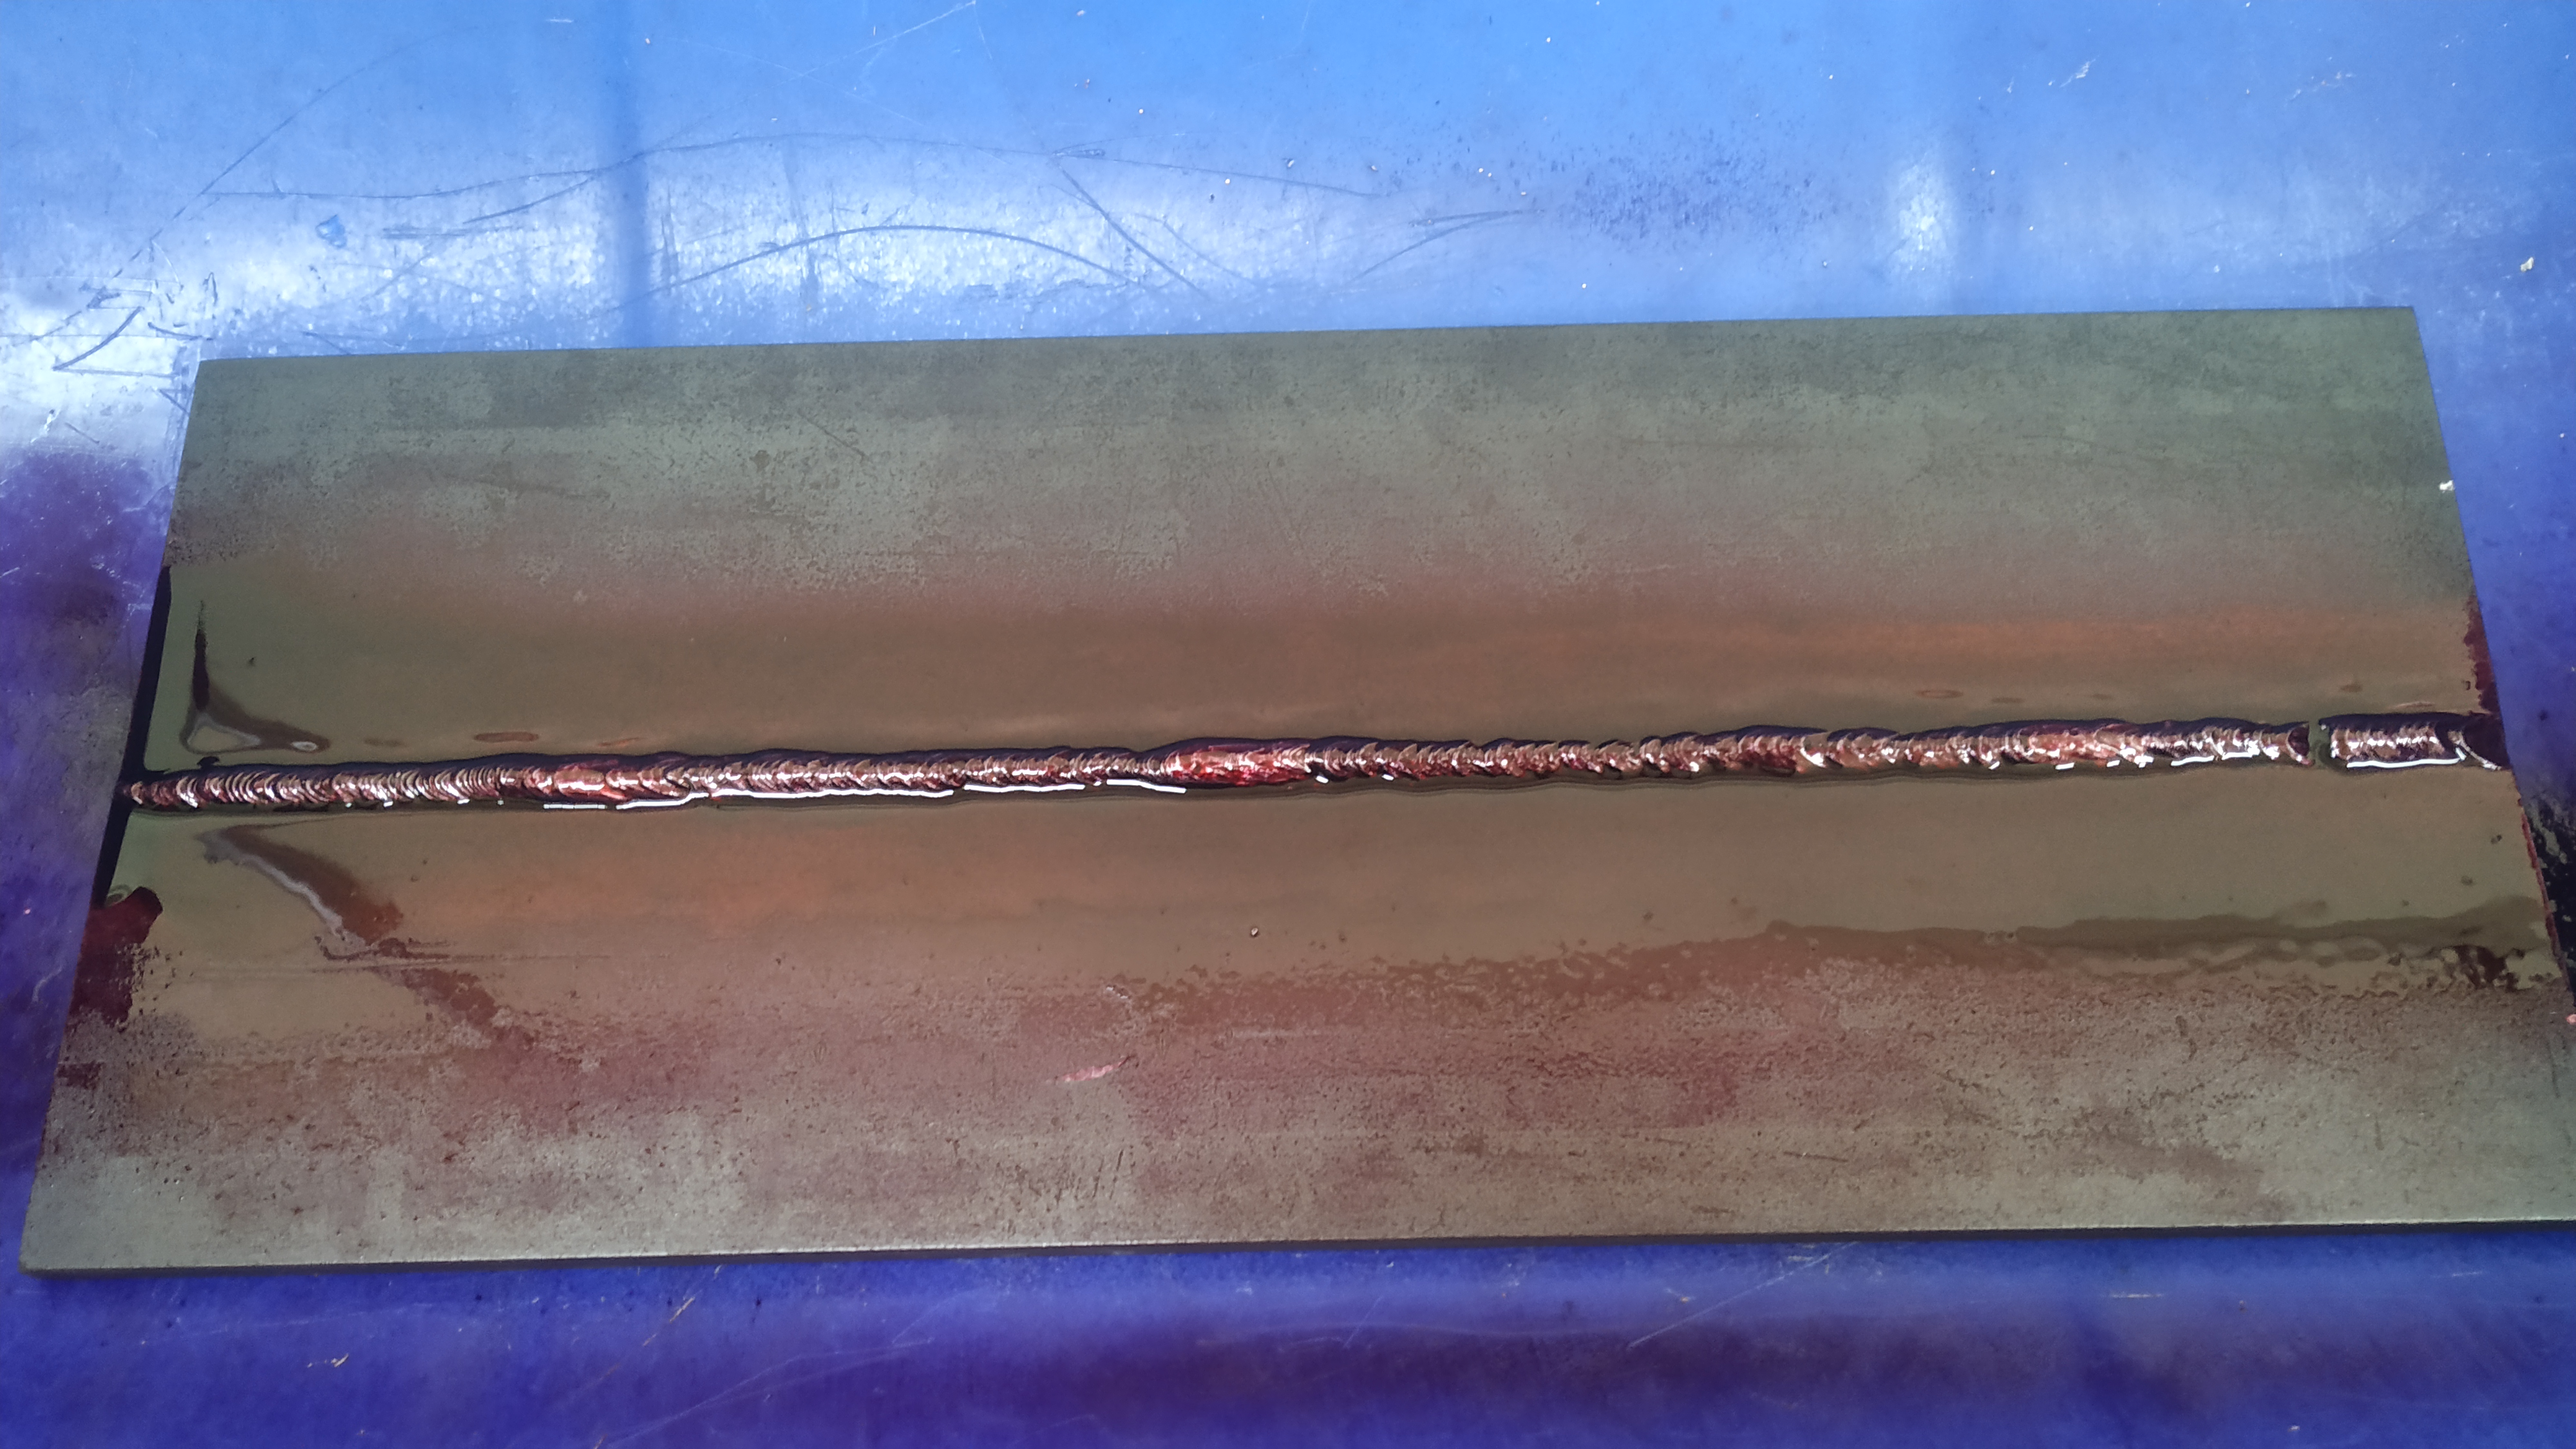
\includegraphics[width=0.65\linewidth]{figuras/aplicacao}
        \caption{Aplicação do LP}
        \label{fig:aplicação-lp}
    \end{subfigure}
    \begin{subfigure}{.5\textwidth}
        \centering
        % include second image
        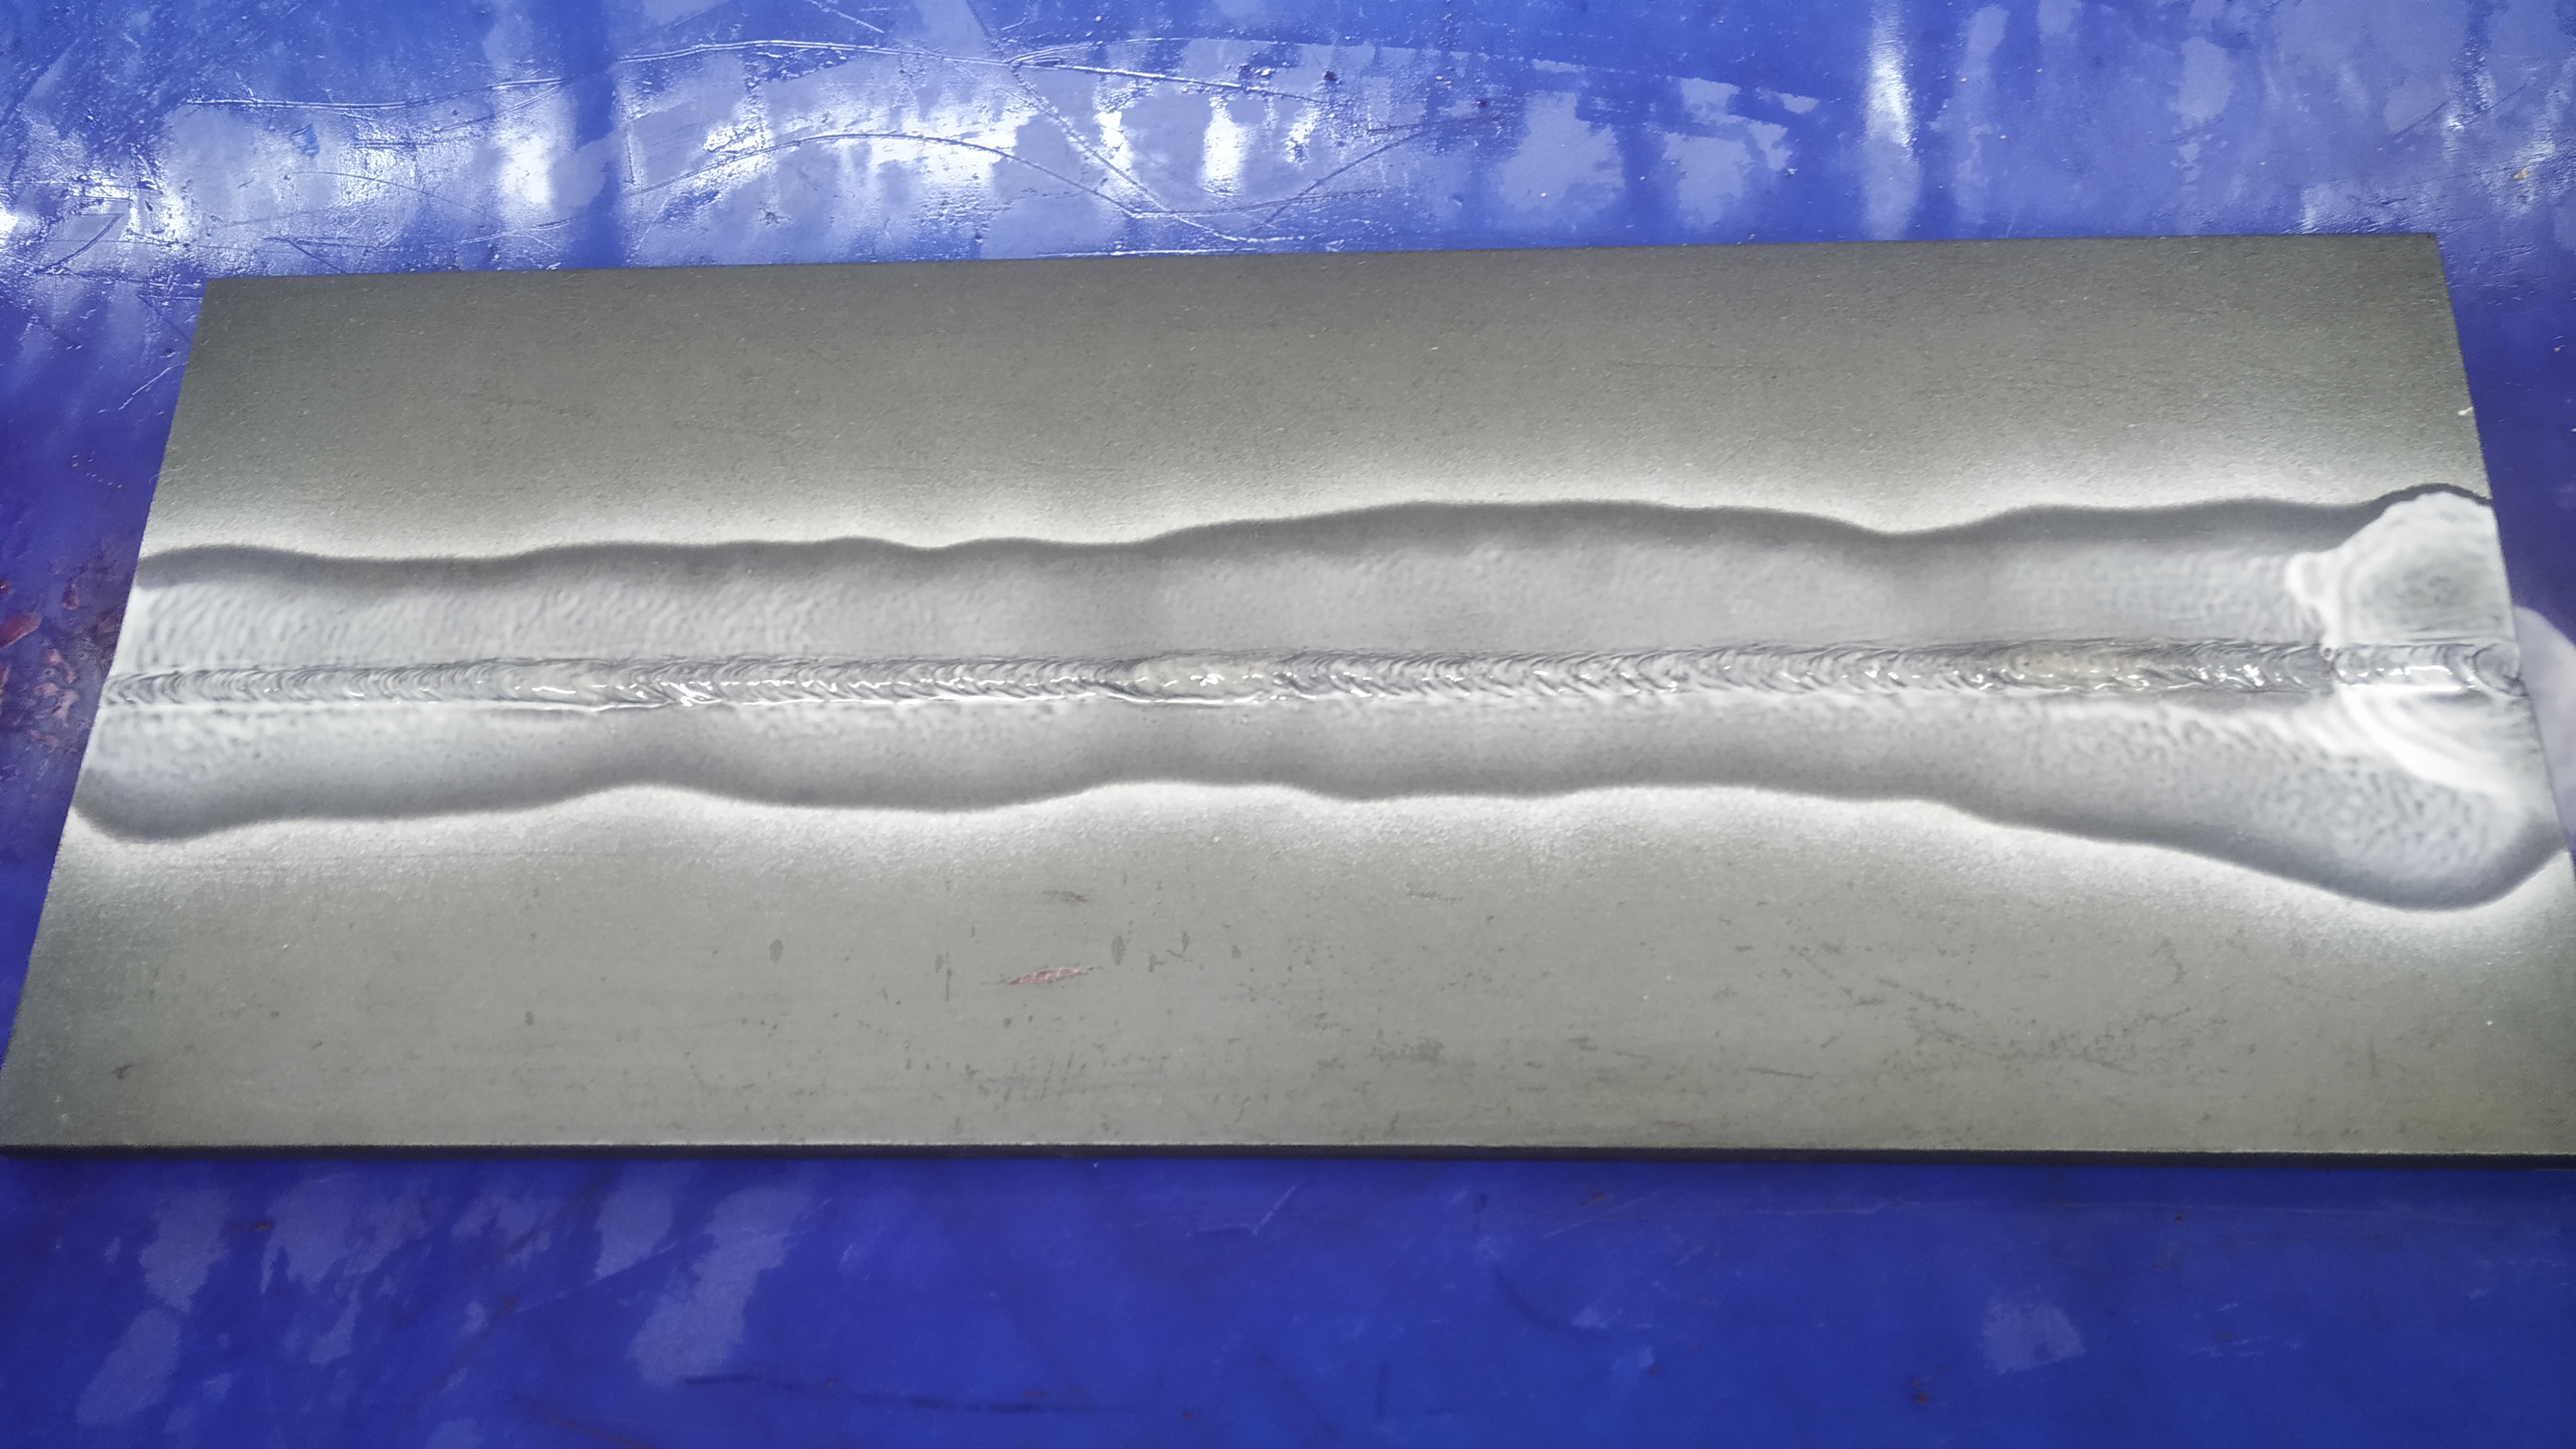
\includegraphics[width=0.65\linewidth]{figuras/aplicacao2}
        \caption{Aplicação do revelador}
        \label{fig:aplicação-revelador}
    \end{subfigure}
    \begin{subfigure}{\textwidth}
        \centering
        % include first image
        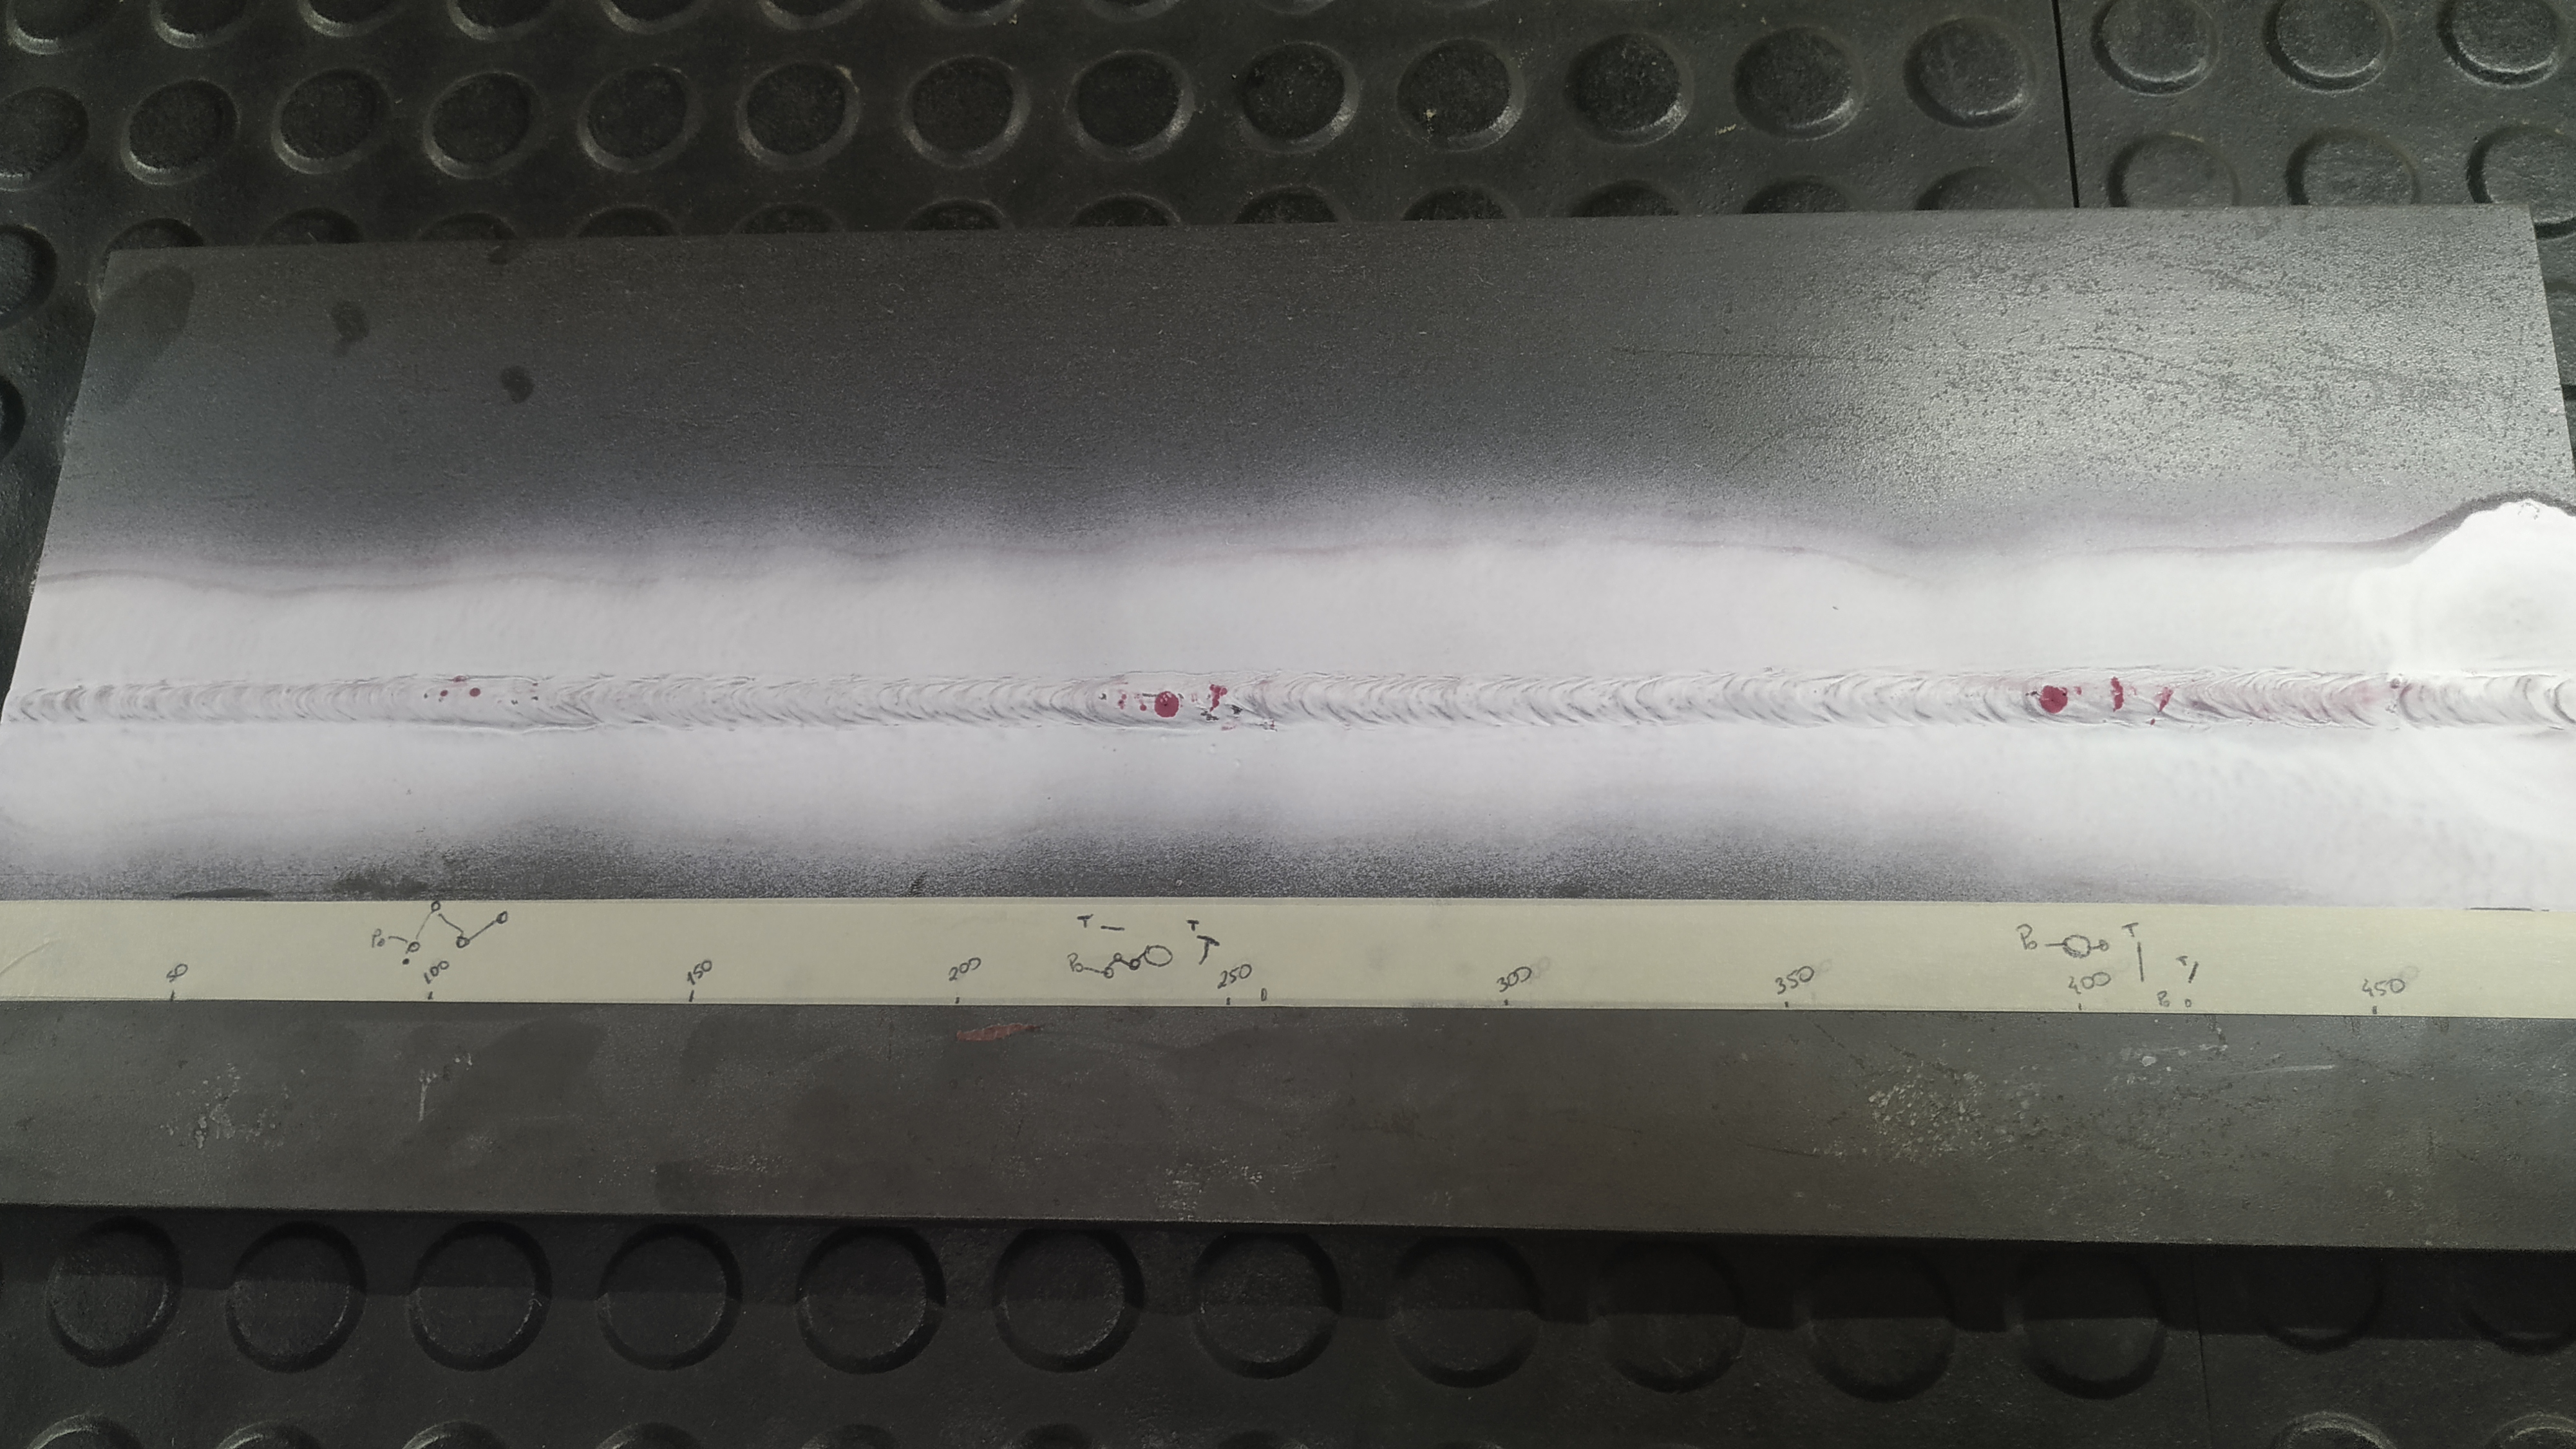
\includegraphics[width=0.82\linewidth]{figuras/aplicacao3}
        \caption{Descontinuidades reveladas}
        \label{fig:fig1-descontinuidades}
    \end{subfigure}
    \caption{Etapas do ensaio de LP.}
    %\caption*{Fonte: Autor}
    \label{fig:fig1}
\end{figure}

\begin{figure}[b!]
    \centering
    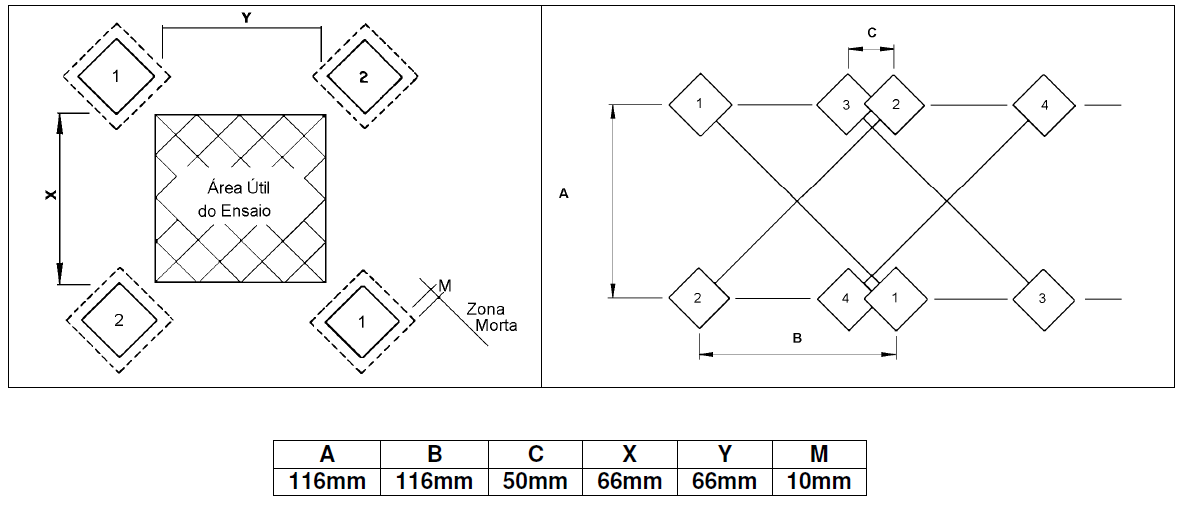
\includegraphics[width = 0.85\linewidth]{figuras/pm-esquema.png}
    \caption{Posicionamento esquemático do Yoke na peça}
    \label{fig:pm-esquema}
\end{figure}

\clearpage
\section{Conclusões}
O ensaio de líquido penetrante é bastante simples de ser realizado e não
requer grande experiência do operador. Também não possui limitações quanto
ao tipo de material, tamanho ou forma das peças a serem ensaiadas.
O ensaio é capaz de revelar descontinuidades extremamente pequenas, porém
só detecta descontinuidades abertas e superficiais.

As descontinuidades foram fáceis de se observar durante a execução da prática
por LP como vistas no anexo \ref{anexo:lp}.


Já o ensaio por partícula magnética é capaz de detectar descontinuidades
superficiais e subsuperficiais até 3mm em materiais ferromagnéticos.
No entanto, a execução do ensaio PM requer grande experiência do operador.

%Devido a essa limitação de experiência, não foi possível observar efetivamente
%as descontinuidades no corpo de prova.







%%%
\clearpage

\appendix
\section{Liquido Penetrante}
\label{anexo:lp}
%\thispagestyle{empty}
%\clearpage
%\hfill
%\thispagestyle{empty}
\clearpage

\section{Partícula Magnética}
\label{anexo:pm}
%\thispagestyle{empty}
%\clearpage
%\hfill
%\thispagestyle{empty}
\clearpage

\printbibliography[heading=bibintoc] % utilização de BiBLaTeX (preferível)
% \bibliography{bib} % utilização de BibTeX
\end{document}
